\documentclass[11pt,reqno,final]{amsart}

\pdfcompresslevel=0
\pdfobjcompresslevel=0

\usepackage[dvipsnames]{xcolor}% adds colors
\usepackage{amsmath, amsthm}% {amsfonts, amssymb}

% New Characters
\usepackage[latin1]{inputenc}%
\usepackage[T1]{fontenc}

\usepackage{MnSymbol}
\usepackage[normalem]{ulem}% underlining

\usepackage[theoremfont, largesc]{newpxtext} % different text,math font
\usepackage{newpxmath}

\makeatletter
\DeclareMathRadical{\sqrtsign}{symbols}{112}{largesymbols}{112}
% \let\sqrt=\undefined
% \DeclareRobustCommand\sqrt{\@ifnextchar[\@sqrt{\mathpalette\@x@sqrt}]}
% \def\@x@sqrt#1#2{%
%  \setbox\z@\hbox{$\m@th#1\sqrtsign{\mkern1mu #2}$}
%  \mkern3mu\box\z@}
\makeatother




% Page Typesetting
\usepackage[final]{microtype}
\usepackage{relsize}
\usepackage[margin=1in]{geometry}
\usepackage{framed}
\usepackage{tikz}

\usepackage{csquotes}

\usepackage{setspace}
\onehalfspacing

\usepackage{hyperref}
\hypersetup{
  final,
  pdftitle={Math 135 - Derivative Tests},
  pdfauthor={Bonventre}, 
  linktoc=page,
  pagebackref,
  colorlinks=true,
  citecolor=PineGreen,
  linkcolor=PineGreen,
  linkbordercolor=PineGreen,
}


% Internal References

\usepackage[inline,shortlabels]{enumitem}

% \numberwithin{equation}{section} 
\numberwithin{figure}{section}

\usepackage[nameinlink,capitalise,noabbrev]{cleveref}

\crefname{equation}{}{} % get \cref to behave as \eqref

% \theoremstyle{plain} % bold name, italic text
\newtheorem{theorem}[equation]{Theorem}%
\newtheorem*{theorem*}{Theorem}%
\newtheorem{lemma}[equation]{Lemma}%
\newtheorem{proposition}[equation]{Proposition}%
\newtheorem{corollary}[equation]{Corollary}%
\newtheorem{conjecture}[equation]{Conjecture}%
\newtheorem*{conjecture*}{Conjecture}%
\newtheorem{claim}[equation]{Claim}%
\newtheorem{question}{Question}

\theoremstyle{definition} % bold name, plain text
\newtheorem{definition}[equation]{Definition}%
\newtheorem*{definition*}{Definition}%
\newtheorem{example}[equation]{Example}%
\newtheorem*{example*}{Example}%
\newtheorem{remark}[equation]{Remark}%
\newtheorem{notation}[equation]{Notation}%
\newtheorem{convention}[equation]{Convention}%
\newtheorem{assumption}[equation]{Assumption}%
\newtheorem{exercise}[question]{Exercise}

% ---------- macros
\newcommand{\set}[1]{\left\{#1\right\}}%
\newcommand{\sets}[2]{\left\{ #1 \;|\; #2\right\}}%
\newcommand{\longto}{\longrightarrow}%
\newcommand{\into}{\hookrightarrow}%
\newcommand{\onto}{\twoheadrightarrow}%

\usepackage{harpoon}
\newcommand{\vect}[1]{\text{\overrightharp{\ensuremath{#1}}}}

\newcommand{\del}{\partial}%

\newcommand{\ki}{\chi}
\newcommand{\ksi}{\xi}
\newcommand{\Ksi}{\Xi}

\newcommand{\dlim}{\displaystyle\lim}

% %%%%%%%%%%%%%%%%%%%%%%%%%%%%%%%%%%%%%%%%%%%%%%%%%%%%%%%%%%%%%%%%%%%%%%%%%%%%%%%%%%%%%%%%%%%%%%%%%%%%

\begin{document}


\begin{center}
        \textbf{\Large Math 135, Calculus 1, Fall 2020}\\[10pt]
        {\large 11-18: Derivative Tests}
\end{center}

\thispagestyle{empty}


\renewcommand{\thesection}{\Alph{section}}

% \vspace{-1pt}

% The \textbf{derivative} $f'(x)$ of a function $y=f(x)$ gives:
% \begin{itemize}
% \item the slope of the tangent line
% \item the instantaneous rate of change of $y$ with respect to $x$
% \end{itemize}


\begin{exercise}
        Suppose the function $f$ on $[0,6]$ has \textbf{derivative} given by the following piecewise-linear function:
        \begin{center}
                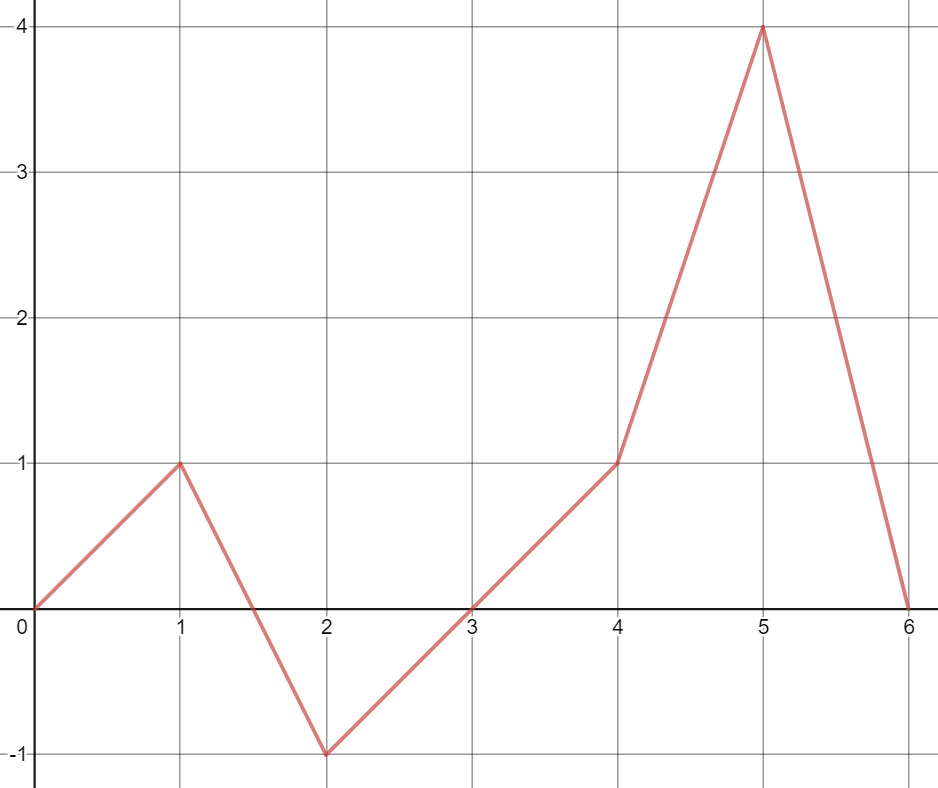
\includegraphics[width=2.5in]{11-18P_g1.png}
        \end{center}
        \begin{enumerate}[(a)]
        \item What are the critical points of $f$?
                \vfill
        \item On what interval(s) is $f$ increasing? decreasing? Make a sign chart for the first deriative.
                \vfill
        \item On what interval(s) is $f$ concave up? down? Make a sign chart for the second derivative.
                \vfill
        \item What are the inflection points of $f$?
                \vfill
        \item Classify the critical points using \textbf{both} the First and Second Derivative Test.
                \vfill
        \end{enumerate}
\end{exercise}

\newpage

\begin{exercise}
        Suppose $g(x)$ is a function which is continuous at all $x \neq 2$ (where it has a vertical asymptote), with \textbf{first} derivative given by
        \[
                g'(x) = \dfrac{(x+4)(x-1)^2}{x-2}.
        \]
        \begin{enumerate}[(a)]
        \item Find all critical points for $g$.
                \vfill
                \vfill
        \item Create a sign chart for the first derivative of $g$, and classify these critical points.
                \vfill
                \vfill
        \item Does $g$ have an absolute max value? absolute min value? Explain.
                \vfill
                \vfill
        \end{enumerate}
\end{exercise}


\begin{exercise}
        Suppose $h(x)$ is a function which is continuous at all $x \neq 2$ (where it has a vertical asymptote), with \textbf{second} derivative given by
        \[
                h''(x) = \dfrac{(x+2)x^3}{(x-3)^2}.
        \]
        \begin{enumerate}[(a)]
        \item Create a sign chart for the second derivative of $h$. Find all inflection points for $h$.
                \vfill
                \vfill
        \item Suppose $x = 1$ is a critical point for $h$. Classify this critical point.
                \vfill
        \end{enumerate}
\end{exercise}



\end{document}
